\part{Vertices}
\frame{\partpage}

\begin{frame}{Position}
	\item Vertices are the basic building blocks of any object
	\pause\item It consists of at least one set of x, y, z coordinates
	\pause\item This represents the position of a vertex in local space
	\pause\item You must provide this x, y, z or the vertex shader will not run
\end{frame}

\begin{frame}{Texture Coordinates}
	\item We use \textbf{UV coordinates} to refer to points in a texture
	\pause\item $u$ axis is horizontal and ranges from 0 (left) to 1 (right)
	\pause\item $v$ axis is vertical and ranges from 0 (bottom) to 1 (top)
	\pause\item (So really just another name for $xy$ coordinates in texture space)
\end{frame}

\begin{frame}{UV coordinates}
\begin{center}
	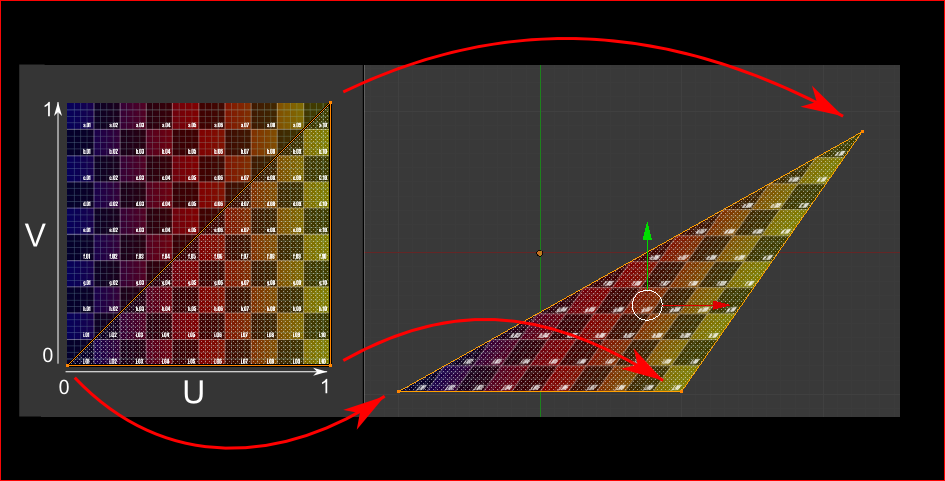
\includegraphics[width=\textwidth]{uv}
\end{center}
\end{frame}